\chapter{Hierarchical Multiple Instance learning} \label{chap:hmill}
In the previous chapter, we summarized machine learning formalism, and we ended with structured data modelling. We want to model specific parts of \emph{JSON} report produced by \emph{CAPEv2} sandbox, as we stated in the introduction. There is a huge amount of information in the behavioural part of the report. Sometimes we can find redundant values in different parts, which shows that the document's structure also keeps some semantics. This chapter describes multiple instance learning as a generalization of the standard learning approach. On top of that is built \emph{HMill} framework, which we describe in the second part of this chapter. At the very end, we describe our modelling use case in detail.

In our experiments, we aim specifically at the hierarchical multiple instance learning (\emph{HMill}) framework defined in \cite{Mandlik2020} because it uses the structure of the input for model computation. The authors proposed a use case of \emph{JSON} modelling with significant results, and we would like to demonstrate the framework's performance on more complex data. In comparison to GNNs approach, \emph{HMill} model has better scalability \cite{Mandlik2020}. 

% In this chapter we describe multiple instance learning as comprehensive approach compared to previus chapter. In the second part we will describe hierarchical multiple instance learning framework as modelling tool to model tree-structured data. Finally, we will address its usage in malware classification and other applications in cyber security field.

\section{Multiple instance learning}
At first, let us describe and define the problem of \emph{Multiple instance learning}, its origin and formalism. This term firstly appeared in \cite{Dietterich1997}, it is not the very first formulation of such problem, that is in \cite{Keeler1991}.

The motivation example in the original paper \cite{Dietterich1997} is formulated in the following way. Imagine we have keys and one door, and some of the keys unlock the door, and some of them do not. Note that we do not have access to the door. We get the keys with labels. In standard learning, our goal is to learn a classification model, which consumes a key and outputs if it can open the door. However, in \emph{multiple instance learning} setting, we receive whole key chains with a various number of keys. Each chain is assigned with a label showing if it contains a key opening the door or not. Our goal is to learn a classification model, which consumes a key chain and outputs if it can open the door. We should not check every single key.

In the figure \ref{fig:mill} we can see basic idea behind \emph{Mill} problem ($I_i$ denote instance). The only significant difference regarding the previous chapter is the definition of an \emph{Example}. 
\paragraph{Example}
We assume a \emph{supervised} learning setting. Our examples consist of two parts - \emph{bag} $b$ and \emph{state} $y$. A state was defined earlier and its meaning is the same, but it is related to a bag and sometimes called \emph{bag label}. \emph{Bag} $b$ is a set of feature vectors $x_i\in\mathcal{X}$, these vectors are called \emph{instances} and usually lives in the standard feature space $\mathbb{R}^{d}$. The cardinality of each bag is $|b| \in \mathbb{N}$ and can be even zero. We assume $b \in \mathcal{B}$ which denotes a \emph{bag space}. \emph{Bag space} might also be seen as $\mathcal{B} = \mathrm{Fin}(\mathcal{X})$ which denotes all finite subsets of $\mathcal{X}$. We can see a standard learning situation described in chapter \ref{chap:classification} corresponds to a \emph{Mill} problem where holds $|b| = 1$.

For the thesis we assume \emph{Mill} classification problem so $|\mathcal{Y}|$ is finite (typically binary classification $\mathcal{Y} \in \{positive, negative\}$). 
% Some researches and even the original paper has one assumption (sometimes called \emph{Standard assumption}). This assumption is about underlying \emph{instance labels} and their relation to \emph{bag labels}. This assumptions is often relaxed \cite{Xu2003} and that is also our case.

\begin{figure}
    \centering
    \subfloat[Standard situation]{
        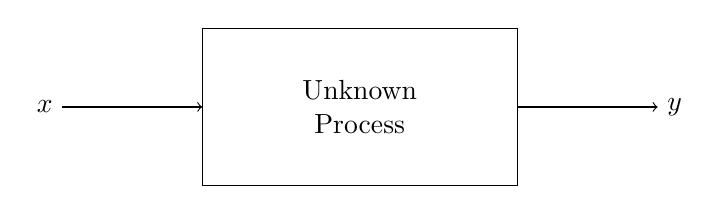
\begin{tikzpicture}
            \node (X) at (-2,1) {$x$};
            \node (Y) at (6,1) {$y$};
            \draw (0,0)rectangle(4,2)node[midway,black,align=center]{Unknown \\ Process};
            \path [->] (X) edge (0,1);
            \path [->] (4,1) edge (Y);
        \end{tikzpicture}
    }
    \par
    \subfloat[Multiple instance situation]{
        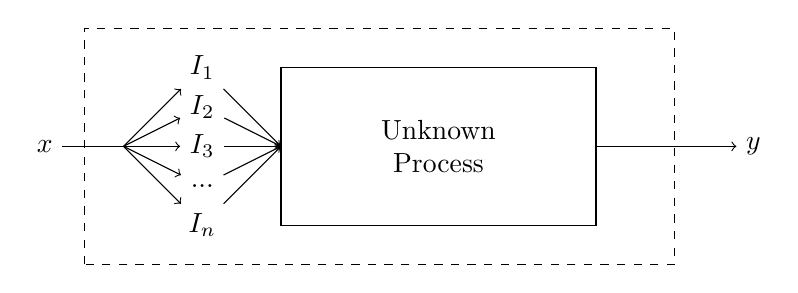
\begin{tikzpicture}
            \node (X) at (-3,1) {$x$};
            \node (Y) at (6,1) {$y$};
            \node (I1) at (-1,2) {$I_1$};
            \node (I2) at (-1,1.5) {$I_2$};
            \node (I3) at (-1,1) {$I_3$};
            \node (I4) at (-1,0.5) {$...$};
            \node (I5) at (-1,0) {$I_n$};
            \draw (0,0)rectangle(4,2)node[midway,black,align=center]{Unknown \\ Process};
            
            \path [-] (X) edge (-2,1);
            \path [->] (-2,1) edge (I1);
            \path [->] (-2,1) edge (I2);
            \path [->] (-2,1) edge (I3);
            \path [->] (-2,1) edge (I4);
            \path [->] (-2,1) edge (I5);
            \path [->] (I1) edge (0,1);
            \path [->] (I2) edge (0,1);
            \path [->] (I3) edge (0,1);
            \path [->] (I4) edge (0,1);
            \path [->] (I5) edge (0,1);
            \path [->] (4,1) edge (Y);
            
            \draw [dashed] (-2.5,-0.5)rectangle(5,2.5);
        \end{tikzpicture}
    } 
    \caption{Supervised learning}
    \label{fig:mill}
\end{figure}

\section{\emph{Mill} problem solutions}
The goal of the \emph{HMill} learning process is identical to that in the standard setting. This section describes three general approaches (paradigms) of solving a \emph{HMill} problem. They are formulated in \cite{Amores2013} as \emph{Instance-Space, Bag-Space} and \emph{Embedded-Space} paradigm.

\subsection{Instance-Space paradigm}
An algorithm in this group infers an \emph{instance-based} classifier $f(x) \in \{1,0\}$ that classifies each instance $x$ in the training set. \emph{Bag-based} classifier is constructed in the way shown in \ref{eq:bagsclas}, where $x_i$ are instances in the bag $b$, $\circ$ denotes an algorithm-specific aggregation operator and $Z$ denotes an optional normalization factor. As we stated earlier, \emph{bag} labels are part of the training set but \emph{instance labels} do not. We have to make some assumptions about the relation between \emph{bag} and \emph{instance} labels, if we want to use method buliding on Instance-space paradigm.

\begin{equation} \label{eq:bagsclas}
    F(b)=\frac{f(x_1)\circ f(x_2)\circ\dots\circ f(x_N)}{Z}
\end{equation}

\subsubsection{Standard assumption}
We assume that each negative bag consists of negative instances only, and each positive bag includes at least one positive instance. An algorithm in this setup aims to aim at instances that make bags positive (we know that at least one in each bag does that).

There are several methods that follow this assumption. The first is \emph{Axis-Parallel Rectangle} used in \cite{Dietterich1997} in drug discovery use case, where $F(b)=\max_{x\in b}f(x)$. Other methods are \emph{Diverse Density} \cite{Maron1998} or MI-SVM \cite{Andrews2003}.

\subsubsection{Collective assumption}
Previous methods tend to look over the fact that the bag label might be influenced by the interaction of features from different instances. Some of them might consider only several instances (or even one) from the whole bag.

\emph{Collective assumption} states that \say{all instances in a bag contribute equally to the bag’s label} \cite{Xu2003}. Methods usually use a training set of instances which is constructed such that each instance inherits its bag's label.

This training set might be used to get an instance-level classifier. A basic approach is to use the SIL algorithm \cite{Bunescu2007}, which train mentioned instance-level classifier using SVM. The bag-level classifier is obtained by \ref{eq:collass}. Another method is Wrapper MI \cite{Frank2003}.

\begin{equation} \label{eq:collass}
    F(b)=\frac{1}{|b|}\sum_{x\in b}f(x)
\end{equation}

\subsection{Bag-Space paradigm}
In this setup, we treat whole bags to learn the classifier. The discriminant learning process is performed in \emph{bag space} directly in contrast to the previous paradigm where we assumed instance-level classifiers.

\emph{Bag space} is a non-vectorial, however we are able to define a distance function $D(b_1,b_2)$, where $b_1$, $b_2$ are bags and the result is representing a measure of their similarity (or distance). Then we can use standard distance-based classifiers such as SVM or K-NN.

Assume, instances lives in \emph{d-dimensional} space such as $\mathbb{R}^{d}$. We can see them as points, so a bag is a set of points. A distance function for two sets of points is well-known problem. Example of distance function is minimal Hausdorff distance \ref{eq:haus}, which denotes distance between closest points of bags $b_1$ and $b_2$ \cite{Wang2000}. We can also use kernel functions $K(b_1,b_2)$ which provide similarity between bags. An example of such kernel might be \ref{eq:kernel}, where $k(x,y)$  denotes instance-level kernel (linear, polynomial\dots) and $p$ is related to the size of the largest bag (in practise found by cross-validation) \cite{Gartner2002}.

\begin{equation} \label{eq:haus}
    D(b_1,b_2)=\min_{x\in b_1, y\in b_2}||x-y||
\end{equation}

\begin{equation} \label{eq:kernel}
    K(b_1,b_2)=\sum_{x\in b_1, y\in b_2}k(x-y)^{p}
\end{equation}

\subsection{Embedded-Space paradigm}
In the Bag-Space paradigm, the goal is to extract global information from bags. That is achieved by defining a distance function which allows us their implicit comparison. In the Embedded-Space paradigm, we extract the information by defining explicit mapping $\mathcal{M}:b\mapsto v$ from the bag space to a custom feature space which summarizes bag characteristics,  $\mathcal{M}$ we call \emph{embedding}. Based on the choice of $\mathcal{M}$, we may distinguish two approaches - \emph{without vocabulary} and \emph{vocabulary-based} methods.

\emph{Without vocabulary} approaches make no differentiation among instances in a bag and aggregates overall statistics from each instance of the bag. An example of such algorithm might be \emph{Simple MI} where the feature vector for a bag is attained by averaging over all instances in it: $\mathcal{M}(b)=\frac{1}{|b|}\sum_{x\in b}x$ \cite{Dong2006}.

\subsubsection{Vocabulary-based methods}
These methods are in the embedded-space category, and the main idea is to find an embedding based on an instance-level classification. However, instance labels are assumed in a different sense than in the Instance-Space paradigm. We often involve an unsupervised way to derive the instance-level classifier, so the semantics of an instance class is missing here. Bag embedding is then determined according to instance classes.

There are three usual components of a \emph{vocalbulary-based method} \cite{Amores2013}. \emph{Vocabulary} $\mathcal{V}$ storing instance-level classes (sometimes rather called concepts). Each concept is defined by an identifier and a set of parameters. These concepts are most often created from clusters of K-means algorithm. Second component is a \emph{mapping function} $\mathcal{M}(b, \mathcal{V})=v$ (embedding) which maps from the \emph{bag space} to  a $k$-dimensional \emph{feature space}, where $k$ denotes the number of concepts. The final component of a \emph{vocabulary-based} method is a standard supervised classifier $\mathcal{G}(v) in \{1,0\}$ which classifies feature vectors in embedded space. Final bag-level classifier results in $F(b)=\mathcal{G}(\mathcal{M}(b,\mathcal{V}))$

We may distinguish several approaches for \emph{vocabulary-based} methods. As an example, we describe \emph{histogram-based} methods. Remaining approaches are \emph{distance-based} and \emph{attribute-based}, for more info we refer to \cite{Amores2013}.

\subsubsection{Histogram-based methods}
$\mathcal{V}$ denotes resulting clusters of chosen clustering algorithm which outputs $K$ classes $C_1,\dots C_K$. $\mathcal{M}$ denotes a histogram of classes for instances in a particular bag: $\mathcal{M}(b,\mathcal{V})=(v_1,v_2\dots,v_K)$, where $v_j=\frac{1}{Z}\sum_{x\in b}f_{j}(x), j=1,\dots,K$, where $f_{j}(x) \in \{1,0\}$ is likelihood that the instance $x$ belongs to the class $C_j$ and $Z$ is a normalization factor. Example of such algorithm is Bag-of-Words \cite{Nowak2006}.

A generalization of all listed paradigms is provided in \cite{Mandlik2020}. The authors stated that all approaches require three essential components - function operation at the instance level $f$ (e. g. \ class classifier), a form of aggregation or pooling $g$ and bag-level classifier $F$. That leads us to the last method we want to describe.

All three functions are composed together to retrieve a prediction. The idea is to optimize everything together. If all functions $f$,$g$ and $F$ are (at least piecewise) differentiable with respect to their parameters, we can use gradient descent optimization. \cite{Pevny2016a, Edwards2017} This approach is very flexible as the whole composition is optimized together in contrast to the previous cases where they are designed separately and later connected. For more, no instance labels are required. They are treated implicitly in an unsupervised manner. An example of such a neural network architecture is demonstrated in \ref{fig:hmill}. Note that there is one $f$ with shared parameters $\Theta_{f}$ over all instances. The pooling function $g$ might be mean or maximum and final layer $F$ after the pooling gets fixed dimension bag representation as input.

\begin{figure}[!ht]
    \centering
    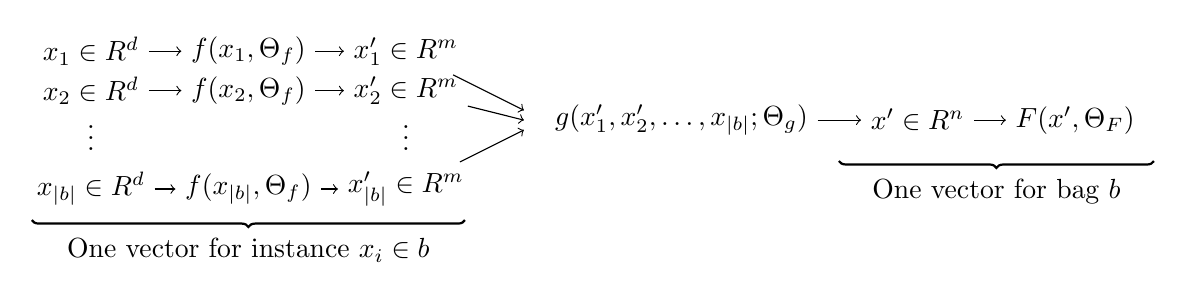
\begin{tikzpicture}
        \node (I1) at (-6,2) {$x_1 \in \mathbb{R}^{d}$};
        \node (I12) at (-4,2) {$f(x_1,\Theta_{f})$};
        \node (I13) at (-2,2) {$x_1' \in \mathbb{R}^{m}$};
        \path[->] (I1) edge (I12);
        \path[->] (I12) edge (I13);
        
        \node (I2) at (-6,1.5) {$x_2 \in \mathbb{R}^{d}$};
        \node (I22) at (-4,1.5) {$f(x_2,\Theta_{f})$};
        \node (I23) at (-2,1.5) {$x_2' \in \mathbb{R}^{m}$};
        \path[->] (I2) edge (I22);
        \path[->] (I22) edge (I23);
        
        \node (Ik) at (-6,1) {\vdots};
        \node (Ik3) at (-2,1) {\vdots};
        
        \node (I3) at (-6,0.25) {$x_{|b|} \in \mathbb{R}^{d}$};
        \node (I32) at (-4,0.25) {$f(x_{|b|},\Theta_{f})$};
        \node (I33) at (-2,0.25) {$x_{|b|}' \in \mathbb{R}^{m}$};
        \path[->] (I3) edge (I32);
        \path[->] (I32) edge (I33);
        
        \node (G) at (1.5,1.125) {$g(x_1',x_2',\dots,x_{|b|};\Theta_{g})$};
        \path[->] (I33) edge (-0.5,1);
        \path[->] (I23) edge (-0.5,1.125);
        \path[->] (I13) edge (-0.5,1.25);
        
        \node (R) at (4.5,1.125) {$x' \in \mathbb{R}^{n}$};
        \path[->] (G) edge (R);
        
        \node (F) at (6.5,1.125) {$F(x',\Theta_{F})$};
        \path[->] (R) edge (F);
        
        
        \draw[thick,decorate,decoration={brace, raise=-3pt}] (-1.25, -0.25) -- (-6.75, -0.25) node[midway,below]{One vector for instance $x_i \in b$ };

        \draw[thick,decorate,decoration={brace, raise=-3pt}] (7.5, 0.5) -- (3.5,0.5) node[midway,below]{One vector for bag $b$ };
        
    \end{tikzpicture}
    \caption{Hierarchical mill model by \cite{Pevny2016a} (image inspired by \cite{Mandlik2020})}
    \label{fig:hmill}
\end{figure}

Demonstration of this approach and its results can be found in \cite{Pevny2016a,Pevny2017, PevnyDedic2020, Mandlik2020, Janisch2020,PevnyKovarik2019a}. The same idea was published independently as \emph{Deep sets} in \cite{Zaheer2018}.

In \cite{Mandlik2020} we can see an application of this approach in an introduced \emph{HMill} framework. Further, we describe this framework.



% \todo{List paradigm and shortly describe and add some examples (prior) of solutions - cite from Amores}
% another examples we can find here - https://www.etsmtl.ca/Unites-de-recherche/LIVIA/Recherche-et-innovation/Publications/Publications-2017/mil_marc_2017.pdf

% \todo{some real world examples (not only pevny and Mandlik).}


% - Prior experiments (Some of them mention here, some of them below in hmill section)
%     Look at applications which are in previous papers above (mandlik, pevny..)
%         \cite{Stiborek2018}

\section{HMill framework}
The idea of the neural net architecture defined in \cite{Pevny2016a} was followed by \cite{Mandlik2020} which led to the formulation of \emph{HMill framework} referring to the \emph{Hierarchical Multiple instance learning framework}. This framework provides general tools for graph-structured data modelling. Both sample and model consist of various type nodes which are structured as a rooted directed tree. The crucial publication for \emph{hmill framework} is \cite{Mandlik2020} where authors firstly formulated this framework and demonstrated its use. In this section, we summarize the most important facts. Should the reader wish to learn more, we recommend original publication \cite{Mandlik2020}.

\subsection{Abstract data nodes}
Firstly, let us summarize basic data nodes in \emph{hmill} framework. The data nodes are used to represent samples. Demonstration of their usage can be seen in figure \ref{fig:irismill}.
%\todo{transform figure to pdf}
\subsubsection{Array node}
Our data consist of some low level observations e.g. \ strings, booleans, vectors, enums\dots Authors call these raw observations - \emph{fragments} and $\mathcal{F}$ denotes the space where they are living. Examples of $\mathcal{F}$ might be Euclidean space $\mathbb{R}^{k}$, linear space $\mathbb{Z}^{2}$ or even all strings over finite alphabet. The only requirement for $\mathcal{F}$ is that there have to exist such mapping $\mathcal{F}\xrightarrow{h}\mathbb{R}^{n}$. The array node is responsible for storing \emph{fragments} $\alpha\in\mathcal{F}$ in following form: $an(\alpha,\mathcal{F},h)$. Sometimes the notation is $an(x)$, where $x=h(\alpha)$ meaning that the trasformation was already made.

\subsubsection{Bag node}
\emph{Bag node} denotes analogy to \emph{bag} in multipliple instance learning $bn(b)$, where $b=\{a_1,\dots,a_{|b|}\}$. 
From the structural point of view, a bag node can be created from a graph node that has:
\begin{enumerate}
    \itemsep0em 
	\item multiple children, which are $an$ with matching $\mathcal{F}$
	\item multiple subtrees $bn_i$ with matching structure\footnote{follows the same schema which is defined later} (nested)
\end{enumerate}
As the instances have to be of the same structure, they form an unordered set in a bag node.

\subsubsection{Product node}
Final node type of \emph{HMill} tree representation of sample is a \emph{product node}. That is defined as $pn(a_1,\dots,a_{l}$, where $l\geq1$ and $a_i$ is representation of some \emph{HMill} tree/subtree - \emph{an,bn} or \emph{ps}. The order of $a_i$ is arbitrary but fixed because each abstract node in it might have different dimensions.

\begin{figure}[h]
    \centering
    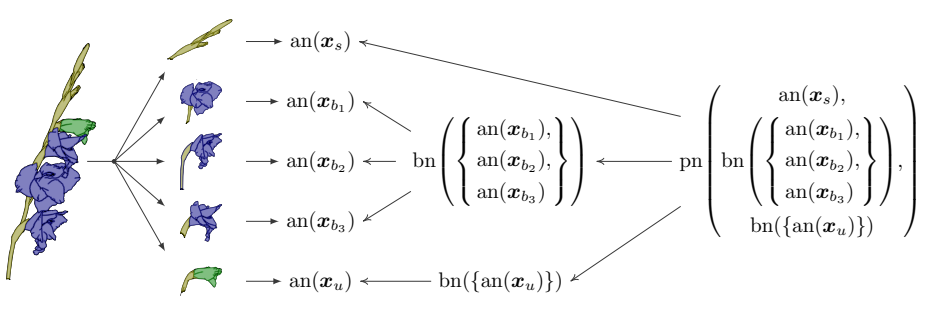
\includegraphics[width=0.9\textwidth]{figures/irismill.png}
    \caption{Representation of the plant specimen in \emph{HMill} framework (source \cite{Mandlik2020})}
    \label{fig:irismill}
\end{figure}

\subsection{HMill schema}
In the \emph{bag node} definition we mentioned that instances in it have to follow the same structure. That is why we define \emph{HMill schema}. Schemas are trees which are mirroring sample trees and for each abstract data node there is a corresponding schema node in the schema structure. 
\begin{itemize}
    \itemsep0em 
    \item \emph{Array schema node} ($as(\mathcal{F'},h')$ - defines fragments space instance $\mathcal{F'}$ and mapping $h'$
    \item \emph{Bag schema node} ($bs(s')$) - defines subschema (subtree) of instances $s'$ specifying structure of instance in bag node
    \item \emph{Product schema node} ($ps(s_1,\dots,s_{l})$) - defines one or more subschemata $s_i$ of subtrees in product node
\end{itemize}

\paragraph{Definition} (Schema matching according to \cite{Mandlik2020}). We say that a sample tree $t$ follows a schema $s$, or matches a schema $s$, provided following conditions hold:
\begin{itemize}
    \itemsep0em 
    \item If $t=an(\alpha,\mathcal{F},h)$ for any $\alpha\in\mathcal{F}$, then $t$ is matching $s$ if and only if $s=as(\mathcal{F},h)$
    \item If $t=bn(\{a_1,\dots,a_k\})$, then $t$ is matching $s$ if and only if $s=bs(s')$ and $\forall i\in\{1,\dots,k\}:t_i$ matches $s'$
    \item If $t=pn(t_1,\dots,t_l)$, then $t$ is matching $s$ if and only if $s=ps(s_1,\dots,s_k)$,$l=k$ and $\forall i\in\{1,\dots,l\}:t_i$ matches $s_i$
\end{itemize}

Note that an empty bag node matches every schema with a bag node in root. If we observe two samples following the same structure and one of them has instances in a specific bag and the second does not, they still might follow the same schema.

\subsection{HMill model}
After we defined nodes and schema, we can take a training set, derive schema matching all examples and create a \emph{HMill} samples ready for learning. 

Following the idea of the tree structure mirroring in the case of schema definition, we define \emph{HMill} model in the same manner. The goal is to create a model based on the schema extracted from our data, which would accept each sample matching the schema on input. Models consist of model nodes. The model nodes are hierarchically nested function, each of which outputs one vector given one abstract data node. If we want to perform prediction for a particular sample, we evaluate functions in subtrees first and then parents. The model root provides the model output. All nodes are piecewise differentiable with respect to their parameters.

\subsubsection{Array model - $am(f)$}
This model transforms the leaves of the sample tree - fragments. We assume that mapping $h$ is already applied for the original fragment, so they are in $\mathbb{R}^m$.  This model is denoted by $f:\mathbb{R}^m\rightarrow\mathbb{R}^n$. We might use any piecewise differentiable mapping, but the authors refer to dense feedforward neural networks.

\subsubsection{Bag model - $bm(f,g,F)$}
A Bag model is motivated by the solution of a multiple instance learning problem provided in \cite{Pevny2016a}. Each bag model can be seen as a multiple instance learning solver for the problem defined by the corresponding bag node and its instances. There are three composed functions - $f$ denotes \emph{instance model}, $g$ denotes \emph{aggregation} and $F$ denotes \emph{bag mapping}. We apply $f$ for each instance/subtree $a_i$ in $bn(a_1,\dots,a_k)$ . All results are input for one or more aggregation functions $g$, and its output is a single vector. Finally, the \emph{bag mapping} $F$ is applied. The output lives in  $\mathbb{R}^d$, where $d$ is the output dimension of a particular multiple instance model. If the bag model is in the root of the tree, $d$ is the overall output dimension of the model. We often use $d=|C|$ as a number of classes. The output is then interpreted as logits of probabilities of classes.

$f$ might be an arbitrarily complex HMill model. Note that all nodes in a bag node have to follow the same schema, so the $f$ is the same for all instances (subtrees), and the output space is of fixed dimension for all subtrees. We might use \emph{max} or \emph{mean} as an aggregation function $g$. Authors of the framework use one or more layer of a feedforward neural network as $F$.

\subsubsection{Product model - $pm(f_1,\dots,f_l,f_p)$}
A product model consists of $l$ submodels and one more final mapping $f_p$. Each of the submodels processes one child of a corresponding product data node. Each product data node can follow a different schema, so each $f_i$ might be different (not like in the bag model). By applying submodels for corresponding product nodes, we get $l$ vectors which might have different dimension. The product model concatenates all vectors, and the result is transformed one or more times by $f_p$.

As all functions in the tree-structured model are at least piecewise differentiable with respect to all parameters, the backpropagation algorithm is adopted in the overall model optimization. Its adaptation we can find in \cite{Mandlik2020}.

% \todo{maybe add image on page 27 in mandlik...}

% schema and matching schema, valid sample
% Hmill models - try to describe it more briefly and connect it to the original idea by Pevny - do not use many images from mandlik but the original iris and the last one to demonstrate the relation to Pevny, or my simplified version

\subsection{Modelling JSON documents using HMill framework}
In the previous chapter, we described several approaches for \emph{JSON} document modelling, here we move on with how the \emph{HMill} framework deals with this problem. The original publication \cite{Mandlik2020} contains even such an approach. The authors presented experimental results for the \emph{IoT device identification} use case, where the data were \emph{JSON} documents.

Assuming that we have a set of \emph{JSON} documents as dataset $\mathcal{T}$ we require one condition to hold. All documents in our dataset have to follow the same structure (same schema), which means the following:
\begin{itemize}
    \itemsep0em 
    \item Given a fixed position in the tree, we know which keys can be found in this particular position in all documents $d\in\mathcal{T}$.
    \item Values of the same key at the same position in all documents $d\in\mathcal{T}$ must follow the same structure.
    \item Arrays at the same position in all documents $d\in\mathcal{T}$ must be empty or contain the same structured objects.
\end{itemize}

Note that a document can follow the same schema even if it is missing some keys. The matching schema might seem too restrictive, but it is widespread that documents used for a single use case follow the same schema. That is true, especially for machine-generated documents.

The \emph{JSON} to \emph{HMill} sample translation is defined on three basic abstract node types. Each leaf of the tree (\emph{JSON} primitive data type) is transformed into an array data node $an(h(\dots))$, $h$ denotes mapping to $\mathbb{R}^n$. The mapping $h$ is identical for all leaves at the same position in the tree across the dataset, and it might be different for different positions. The product data node is used to model \emph{JSON} object. Because the product node accepts an ordered set, the keys in the \emph{JSON} object have to be ordered. Finally, \emph{JSON} arrays are modelled as bag data nodes. The translation is demonstrated in the figure \ref{fig:jsonhmill}.

%\todo{image of JSON document I should redraw}

\begin{figure}[h]
    \centering
    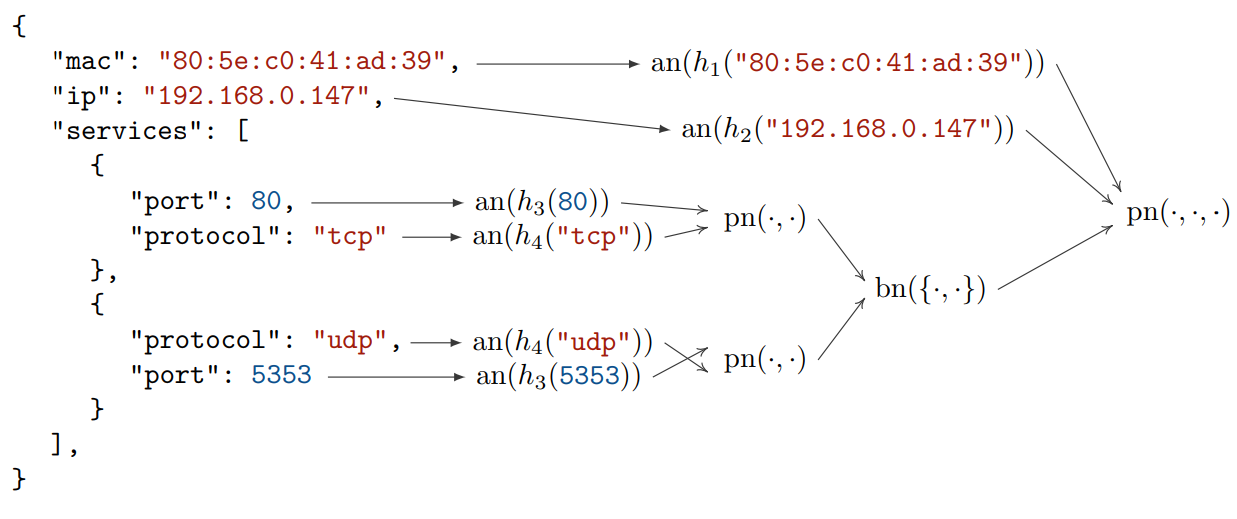
\includegraphics[width=0.9\textwidth]{figures/translation.png}
    \caption{Translation of \emph{JSON} document in \emph{HMill} data nodes (source \cite{Mandlik2020})}
    \label{fig:jsonhmill}
\end{figure}

The authors of the framework stated that the model is taking into the game even the structure which exceeds the \emph{flattening} approach. Compared to the rule-based approaches, the framework can learn more complex hypotheses because chosen aggregation can substitute various hand-defined rules. The \emph{HMill} framework was used in the IoT device identification use case \cite{Mandlik2020}, which was a dataset of \emph{JSON} documents modelled for multinomial classification. Reported accuracy is $96$~\%. Authors experimented even in different setup for a general graph inference to demonstrate the generality of the \emph{HMill} framework.


\section{\emph{CAPEv2} classification}
The goal of the thesis is to create a classifier that classifies signatures based on behavioural features observed during dynamic analysis.

\subsection{Behavioural features}
After further look at the \emph{behavior} part of \emph{report.json} and their size we start with \emph{summary} and \emph{enhanced} part. The reason is that other parts are quite comprehensive, and we would not be able to train the model with the hardware resources we have. Those two are sufficient for a comprehensive look at malware behaviour as they include the most important features mentioned in \ref{chap:analysis} (API calls, commands\dots). In \emph{summary} part, we have unordered lists of these features. However, in \emph{enhanced} part, there are sequences of actions with a timestamp.

If the model is still too complex to train under our conditions, we omit the \emph{enhanced}, which is much more sparse and longer than \emph{summary}. We would lose the information about the order of events.

\subsection{Signature classes}
The signatures are usually assigned based on some atomic fact, such as some API call in the log. Let us call that \emph{true cause} of signature. It can be one or more patterns seen in the behavioural log. The implementation of a signature is deterministically detecting its cause. If the cause is detected, the signature is added to the \emph{JSON} log (see the whole process in \ref{chap:analysis}.

We can consider the \emph{copies self} signature example. If the same file as the analyzed one is among dropped files in the report, we will find \emph{copies self} signature in \emph{report.json}.

An example of a signature entry in original \emph{JSON} log could be seen in \ref{app:signatures}. The most important aside from the \emph{name} and \emph{description} is the field \emph{data} which sometimes contains the cause.

\subsubsection{Categorization}
For modelling and model explaining, we want to categorize signatures according to two factors. The first is the cause, which creates groups such as API calls, processes, dropped files\dots. The cause is determined according to the signature's implementation (typically in Python). In \ref{app:signatures} we can see a simple example of implementation of \emph{antidebugsetunhandledexceptionfilter} signature, which is just checking the presence of a specific API call.

The second factor is the fact if the cause is directly presented among our features. For instance, if the signature implementation uses API calls, the API call list is directly in the log. If it uses the entropy of dropped files, it is not directly in the output.

The categorization may help us with the structure of the result discussion and further reasoning. We expect that models for different categories might have different accuracy.

Specific signatures for modelling will be chosen according to their frequency in the dataset. All the details about chosen signatures and even mentioned groups will be described in the next part of the thesis.

\subsection{Model}
We want to train a binary classifier that predicts the presence of a particular signature according to behavioural features.

emph{Hmill} framework API is designed generally, so it is not accepting \emph{JSON} documents directly. For this purpose, we use \emph{JsonGrinder} library, which accepts an array of \emph{JSON} documents and produce \emph{HMill} schema. The schema is then used to create \emph{HMill} abstract data type tree and model. Example of a schema, and implied \emph{HMill} model for our data is in attachment (\ref{app:attach}).

%---------------------REMAINING-------------------------------------
% \todo{I have to mention some citations the theory I built on top of Mandlik and Amores!}
% \todo{image of standard setting vs mill setting} \todo{if we would like to have some fancy figure we can try something with keys}


% HMILL:
% - assumptions - https://en.wikipedia.org/wiki/Multiple_instance_learning (Be aware, I think those are not true all at once...), also algorithm list is presented, could be mentioned, and other interesting references like problem generalization
% - between modern approaches mention adapting of single instance algorithms

% Previous connection
% - We focus on structured data and our tool is hmill, let's describe it
% Way through this chapter
% - multiple instance learning
% - hierarchical mill
% - prior
%     - Prior in various fields
%     - Prior in cybersec
% Next connection
% - Not necessary, but can connect to next chapter slightly (we want to explain this kind of model)

% Stand on Madlik chapter, his citations (be aware), somol and Pevny


% - GOALS 
% - Learn the hierarchical multiple instance learning framework (HMill)
% - describe theory, connect it to classical approach
% - Usual usage of this type of learning - classification, regression...
% - Our usecase and experiments with this kind of learning in malware classification field (prior)